\subsection{Análisis cuantitativo del error}

Antes de ver los resultados, hagamos un análisis de los casos de prueba que tendremos en cuenta.

\begin{itemize}
    \item \texttt{darthvader}. El primer video contiene una cámara fija y un objeto moviendose a una velocidad relativamente lenta, con su entorno quieto. 
    \item \texttt{ff6}. Este es un video que contiene (a pesar de su corta duración), 6 tomas en escenarios totalmente distintos. Algunos escenarios presentan mucho movimiento, otros estan prácticamente quietos. Este es un video muy interesante para analizar porque es esperable que los algoritmos de interpolación en los que importa sobre todo información local (vecinos más cercanos, interpolación lineal fragmentaria) funcionen mejor que aquellos que toman información global (splines). Analizaremos todo esto más adelante. 
    \item \texttt{motocross}. En este video la cámara se mueve a gran velocidad, siguiendo a un objeto (una moto) que se encuentra más o menos centrada a lo largo de todo el video. 
    \item \texttt{penal}. En este video la cámara está nuevamente fija, pero ahora hay un objeto que se mueve a velocidad medianemente rápida (pateador y arquero) y otro objeto que se mueve a una velocidad muy alta (pelota); mientras que todo el entorno se encuentra quieto. 
\end{itemize}

Elegimos estos videos porque creemos que representan las posibles situaciones o combinaciones que puede presentar un video de la vida real. No elegimos videos confeccionados a mano para analizar casos borde o extremos porque creemos que el análisis más interesante que se puede hacer está alrededor de casos reales, que son finalmente sobre los cuales se aplicarán estos algoritmos.

La métodología de experimentación fue la siguiente: extrajimos 1,2,4 u 8 cuadros por medio de cada video (utilizando el script \texttt{videoToTextfile.py}) y luego lo interpolamos con nuestros algoritmos. Finalmente, utilizando un script hecho por nosotros, comparamos los valores de los píxeles del video original contra los interpolados por nosotros. 

Elegimos esa cantidad de cuadros porque más de 8 cuadros se torna demasiado para interpolar, dado que se pierden muchos detalles del video original y el error se torna realmente alto (ya sucede eso con 8 cuadros).

Por último, para analizar el algoritmo de Splines utilizamos bloques de 4, 8 y 12 cuadros porque, nuevamente, si los bloques eran más grandes el video comenzaba a tener importantes artifacts (ver sección \ref{subsec:cualitativo}) y entonces nos pareció adecuado poner 12 como el tamaño máximo de bloque a tomar (ya en algunos videos 12 es demasiado y el resultado es de mala calidad). Esto se debe a la localidad vs. globalidad de la que hablamos antes, dado que si los frames de un video cambian mucho a lo largo del tiempo, tomar en cuenta frames lejanos a la hora de interpolar es contraproducente.

Sin más aclaraciones que hacer, pasemos a ver y analizar los resultados que obtuvimos.


\begin{figure}[H]
\centering
\begin{minipage}{0.35\textwidth}
    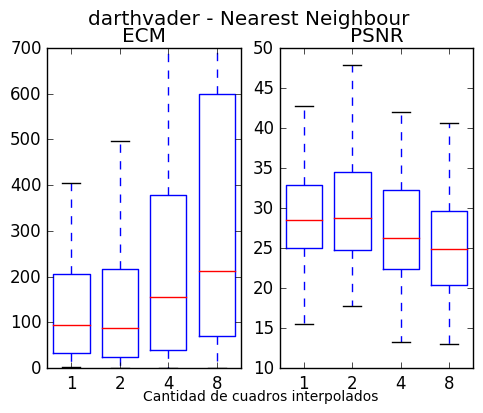
\includegraphics[width=1\textwidth]{imgs/resultados_error/darthvader_0.png}
\end{minipage}%
\begin{minipage}{0.35\textwidth}   
    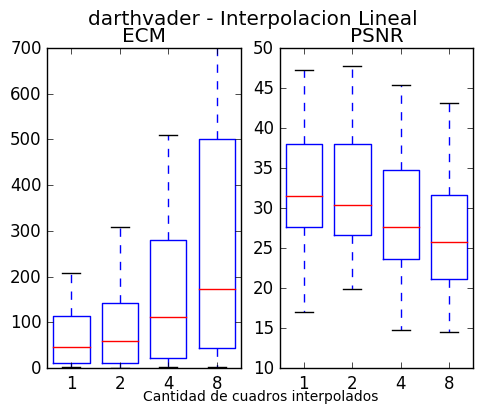
\includegraphics[width=1\textwidth]{imgs/resultados_error/darthvader_1.png} 
\end{minipage}
\end{figure}
\begin{figure}[H]
\centering
\begin{minipage}{0.33\textwidth}   
    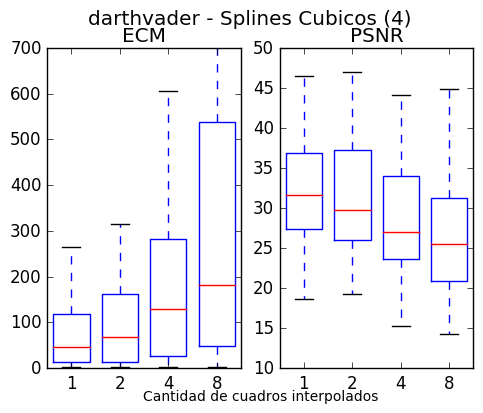
\includegraphics[width=1\textwidth]{imgs/resultados_error/darthvader_2.png} 
\end{minipage}\hfill
\begin{minipage}{0.33\textwidth}   
    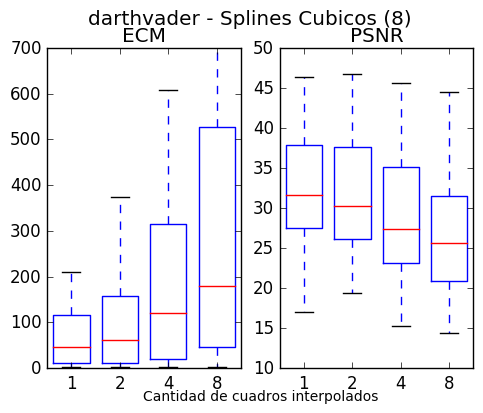
\includegraphics[width=1\textwidth]{imgs/resultados_error/darthvader_3.png} 
\end{minipage}\hfill
\begin{minipage}{0.33\textwidth}   
    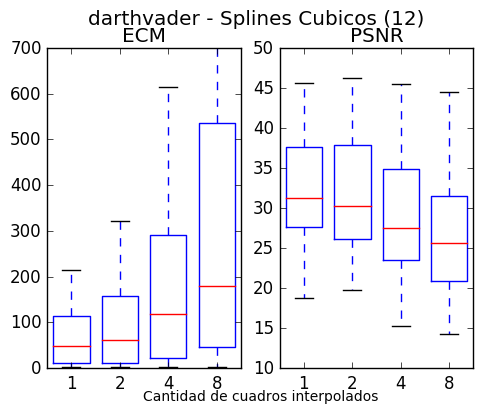
\includegraphics[width=1\textwidth]{imgs/resultados_error/darthvader_4.png} 
\end{minipage}
\label{fig:errdarthvader}
\caption{\footnotesize Resultados del cálculo de ECM y PSNR para cada algoritmo en el video \texttt{darthvader}. Para Splines cúbicos se indica además el tamaño de los bloques utilizados.}
\end{figure}


\begin{figure}[H]
\centering
\begin{minipage}{0.35\textwidth}
    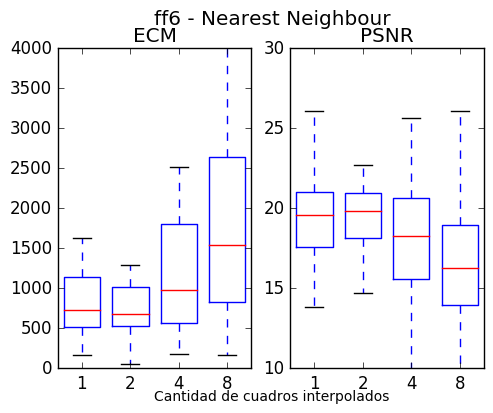
\includegraphics[width=1\textwidth]{imgs/resultados_error/ff6_0.png}
\end{minipage}%
\begin{minipage}{0.35\textwidth}   
    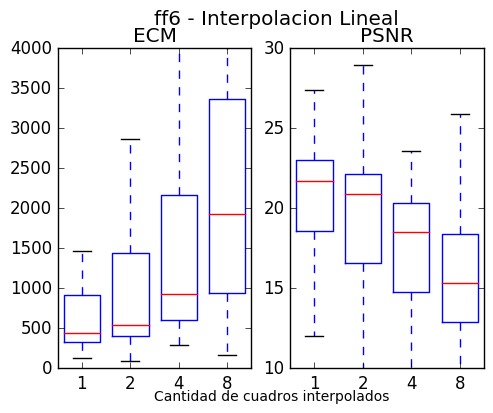
\includegraphics[width=1\textwidth]{imgs/resultados_error/ff6_1.png} 
\end{minipage}
\end{figure}
\begin{figure}[H]
\centering
\begin{minipage}{0.33\textwidth}   
    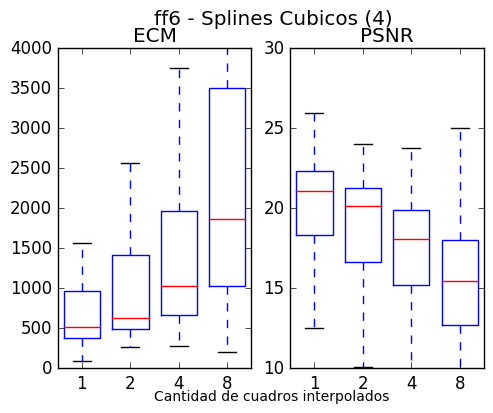
\includegraphics[width=1\textwidth]{imgs/resultados_error/ff6_2.png} 
\end{minipage}\hfill
\begin{minipage}{0.33\textwidth}   
    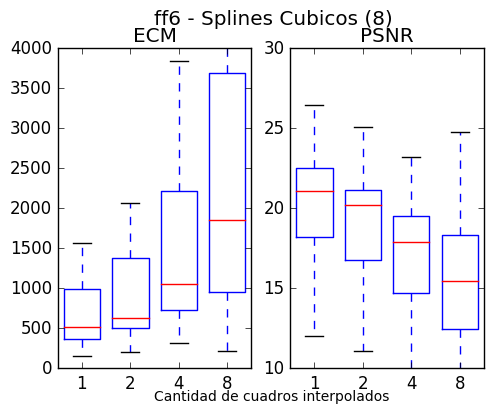
\includegraphics[width=1\textwidth]{imgs/resultados_error/ff6_3.png} 
\end{minipage}\hfill
\begin{minipage}{0.33\textwidth}   
    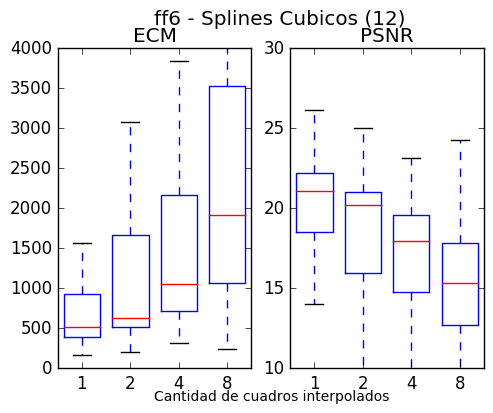
\includegraphics[width=1\textwidth]{imgs/resultados_error/ff6_4.png} 
\end{minipage}
\label{fig:errff6}
\caption{\footnotesize Resultados del cálculo de ECM y PSNR para cada algoritmo en el video \texttt{ff6}. Para Splines cúbicos se indica además el tamaño de los bloques utilizados.}
\end{figure}


\begin{figure}[H]
\centering
\begin{minipage}{0.35\textwidth}
    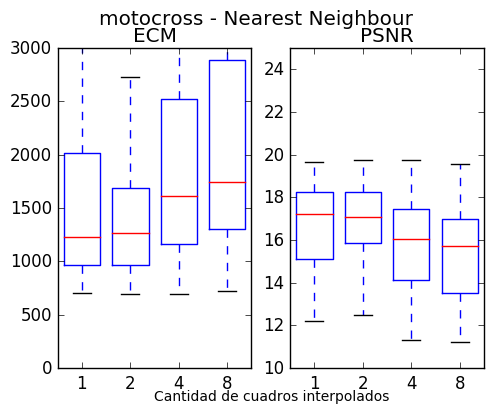
\includegraphics[width=1\textwidth]{imgs/resultados_error/motocross_0.png}
\end{minipage}%
\begin{minipage}{0.35\textwidth}   
    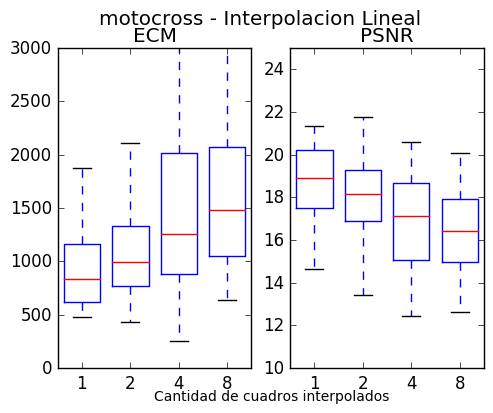
\includegraphics[width=1\textwidth]{imgs/resultados_error/motocross_1.png} 
\end{minipage}
\end{figure}
\begin{figure}[H]
\centering
\begin{minipage}{0.33\textwidth}   
    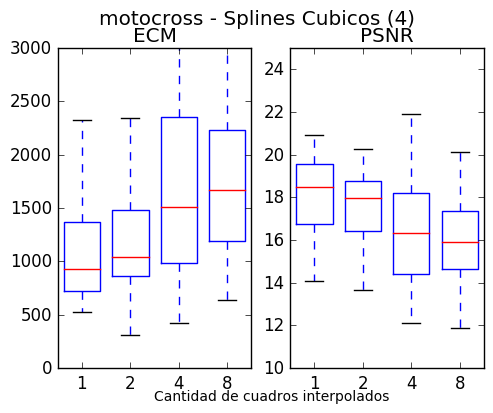
\includegraphics[width=1\textwidth]{imgs/resultados_error/motocross_2.png} 
\end{minipage}\hfill
\begin{minipage}{0.33\textwidth}   
    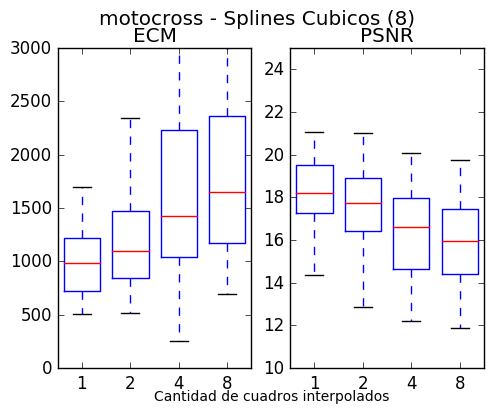
\includegraphics[width=1\textwidth]{imgs/resultados_error/motocross_3.png} 
\end{minipage}\hfill
\begin{minipage}{0.33\textwidth}   
    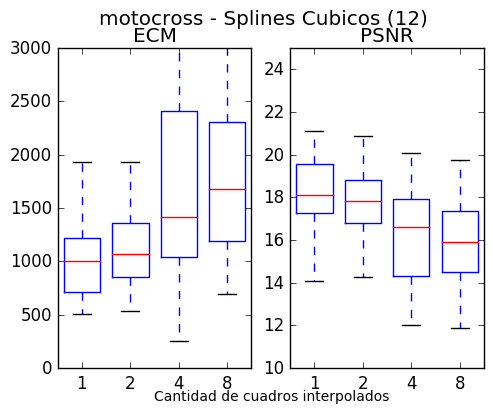
\includegraphics[width=1\textwidth]{imgs/resultados_error/motocross_4.png} 
\end{minipage}
\label{fig:errmotocross}
\caption{\footnotesize Resultados del cálculo de ECM y PSNR para cada algoritmo en el video \texttt{motocross}. Para Splines cúbicos se indica además el tamaño de los bloques utilizados.}
\end{figure}


\begin{figure}[H]
\centering
\begin{minipage}{0.35\textwidth}
    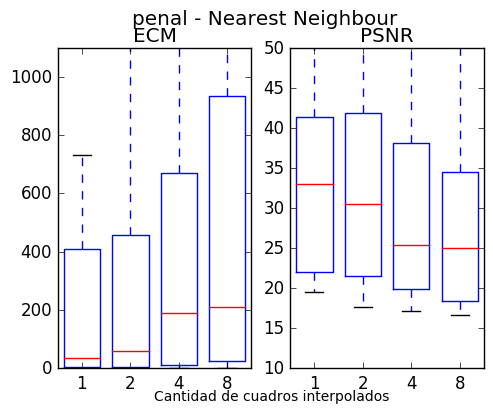
\includegraphics[width=1\textwidth]{imgs/resultados_error/penal_0.png}
\end{minipage}%
\begin{minipage}{0.35\textwidth}   
    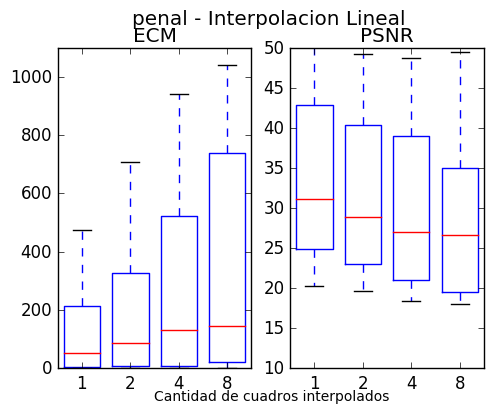
\includegraphics[width=1\textwidth]{imgs/resultados_error/penal_1.png} 
\end{minipage}
\end{figure}
\begin{figure}[H]
\centering
\begin{minipage}{0.33\textwidth}   
    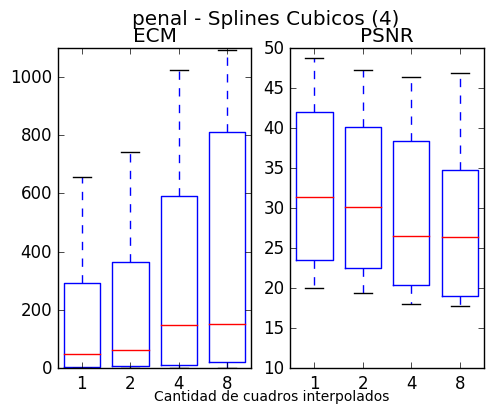
\includegraphics[width=1\textwidth]{imgs/resultados_error/penal_2.png} 
\end{minipage}\hfill
\begin{minipage}{0.33\textwidth}   
    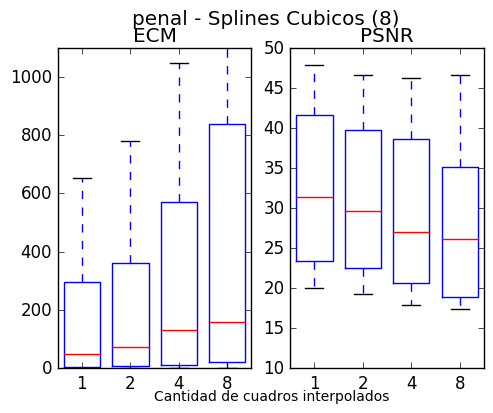
\includegraphics[width=1\textwidth]{imgs/resultados_error/penal_3.png} 
\end{minipage}\hfill
\begin{minipage}{0.33\textwidth}   
    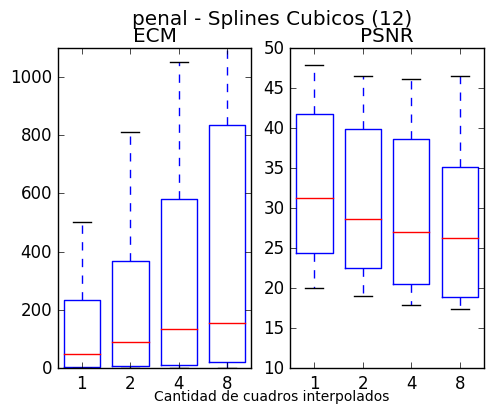
\includegraphics[width=1\textwidth]{imgs/resultados_error/penal_4.png} 
\end{minipage}
\label{fig:errpenal}
\caption{\footnotesize Resultados del cálculo de ECM y PSNR para cada algoritmo en el video \texttt{penal}. Para Splines cúbicos se indica además el tamaño de los bloques utilizados.}
\end{figure}

Antes de analizar los resultados, vale la pena explicar los gráficos que aparecen en las páginas anteriores. Cada boxplot representa los errores (en ECM y PSNR respectivamente) de todos los frames del video. Luego analizaremos dentro de cada video porqu\'e a veces el error es más alto y porqu\'e es más bajo, pero para este análisis en general nos bastará con los boxplots.

Además, vale la pena explicar en que se basan el ECM y el PSNR. El ECM (Error Cuadrático Medio) se calcula como el promedio de todos los errores al cuadrado. Por lo tanto, a más alto, más error. Para este trabajo, consideraremos que un error bajo será un ECM menor a 25, y error medio será ECM menor a 400 (dado que representan diferencias de 5 y 20 respectivamente).

El PSNR (Peak Signal-to-Noise Ratio), se define como $PSNR = 10 \log_{10}(\frac{255^2}{ECM})$. Por lo tanto, a más alto, menos error tendrá la imagen. Puede pensarse como una suerte de ECM normalizado. Usando los mismos números de antes, cosideraremos que el error es bajo si el PSNR es mayor a 35 y que es medio si es mayor a 22 (pero menor a 35).

\subsubsection{\texttt{darthvader}}

Lo primero que podemos notar (muy esperable) es que el error aumenta cuando se intentan interpolar más cuadros. Esto se debe a que se intenta obtener más cantidad de cuadros a partir de una cantidad de datos menor, lo cual obviamente deteriorará la calidad del video.

Lo segundo que notamos es que, mientras el algoritmo de nearest neighbour tiene un error relativamente grande, los algoritmos de interpolación lineal y splines cúbicos (con todos los tamaños de bloque) presentan resultados muy similares. 
Creemos que esto se debe a la lentitud con la que transcurren los hechos en el video provoca que cualquier interpolación razonable de los valores de buenos resultados. 


\subsubsection{\texttt{ff6}}

En este caso, al igual que antes y al igual que en todos los videos que analizaremos, el error aumenta cuando se intentan interpolar más cuadros.


A diferencia que en el video anterior, en este caso se nota una diferencia entre los m\'etodos que utilizamos. Nearest neighbour, como siempre, es el peor, teniendo errores muy altos (dado que los cambios de escenarios en este video son bruscos, un frame puede no tener nada que ver con su anterior).


Luego, podemos ver que la interpolación lineal tuvo mejor performance que los splines cúbicos. La razón de eso es probablemente que, al ser un video que tiene cambios muy abrutpos de escenarios, es mucho mejor obtener los cuadros interpolados con la información lo más local posible, dado que cuadros lejanos tienen muy poco que ver.

Sin embargo, cuantos cuadros se tomen en el spline no afecta demasiado al error. Esto puede explicarse porque los escenarios son relativamente inmóviles, entonces la cantidad de cuadros que se tomen (mientras sean acotados) no debería afectar demasiado porque no agregan información nueva.

\subsubsection{\texttt{motocross}}

Como siempre, el error aumenta cuando se intentan interpolar más cuadros.

En este video sucede algo similar al anterior. Nearest neighbour es el peor porque el video se mueve muy rápido, un frame tiene poco que ver con el anterior. Nuevamente, la interpolación lineal tuvo mejor performance que los splines cúbicos. La razón de esto es la misma que la de antes: al ser un video que se mueve muy rápido, es mejor interpolar con información local que con información global.

Finalmente, podemos notar una diferencia con el video anterior. Podemos observar en la figura \ref{fig:errmotocross} como a más grande es el bloque que se toma para hacer splines cúbicos, más grande es el error. Puede verse que para un tamaño de bloque de 4 frames, el error cuadrático medio es aproximadamente 900, para un bloque de 8 frames de 950 y para uno de 12 es de 1000. 


Este hecho justifica nuestra explicación de porque en el video \texttt{ff6} el tamaño de los bloques no afectó tanto, dado que en este caso tomar bloques más grandes sí agrega nueva información, que sin embargo es perjudicial para el resultado, porque como todo se mueve muy rapidamente, la información nueva altera y distorsiona los resultados.

\subsubsection{\texttt{penal}}

Este es un video muy interesante para analizar. Primero, recordemos que en todo momento la mayor parte del video se encuentra quieta, mientras que algunos objetios que ocupan poca parte de la pantalla se mueven. 

Esto produce que (cuando hay que interpolar 1 o 2 cuadros) el error cuadrático medio se minimice con el algoritmo de vecino más cercano. Esto se debe a que como la mayor parte del video esta quieta, al interpolar con vecino mas cercanos, nos aseguramos que el error en estos lugares sea mínimo, y en las regiones del video que se mueven, el error tambi\'en será relativamente pequeño.

Además, al interpolar 1 o 2 cuadros, el error al usar splines (con cualquier tamaño de bloques) es menor que el de interpolación lineal. Una posible explicación para esto es que splines se adapta mejor que la interpolación lineal fragmentaria a los movimientos rápidos del video, manteniendo la exactitud de los pixeles que cambian poco, con lo cual puede sacarle ventaja.

Ahora bien, cuando se intentan interpolar 4 u 8 cuadros, la situación es muy distinta. Aquí el error de el algoritmo nearest neighbour sube mucho, sobrepasando al de interpolación lineal y splines cúbicos, que estan prácticamente empatados.

Explicar esto no es dificil: al tener que interpolar más cuadros, nearest neighbour empieza a aumentar su error dado que repetir un cuadro muchas veces conlleva bastante error en las partes del video de alto movimiento, dado que el error se arrastra por muchos cuadros. Los algoritmos de interpolación lineal y splines, al utilizar la información mas inteligentemente, son mas \emph{resilientes} a la falta de información, lo cual les permite sobrepasar en rendimiento (con respecto al error) al
algoritmo de nearest neighbour cuando hay que interpolar muchos cuadros.

\subsubsection{Análisis del error a lo largo del tiempo}

Para finalizar con el análisis cuantitativo del error de los algoritmos, nos propusimos analizar como varía el error de nuestra interpolación a lo largo del tiempo para un video dado. Para ello, utilizamos el video \texttt{darthvader}, interpolando 1 cuadro entre dos cuadros consecutivos. Veamos los resultados.

\begin{figure}[H]
    \centering
    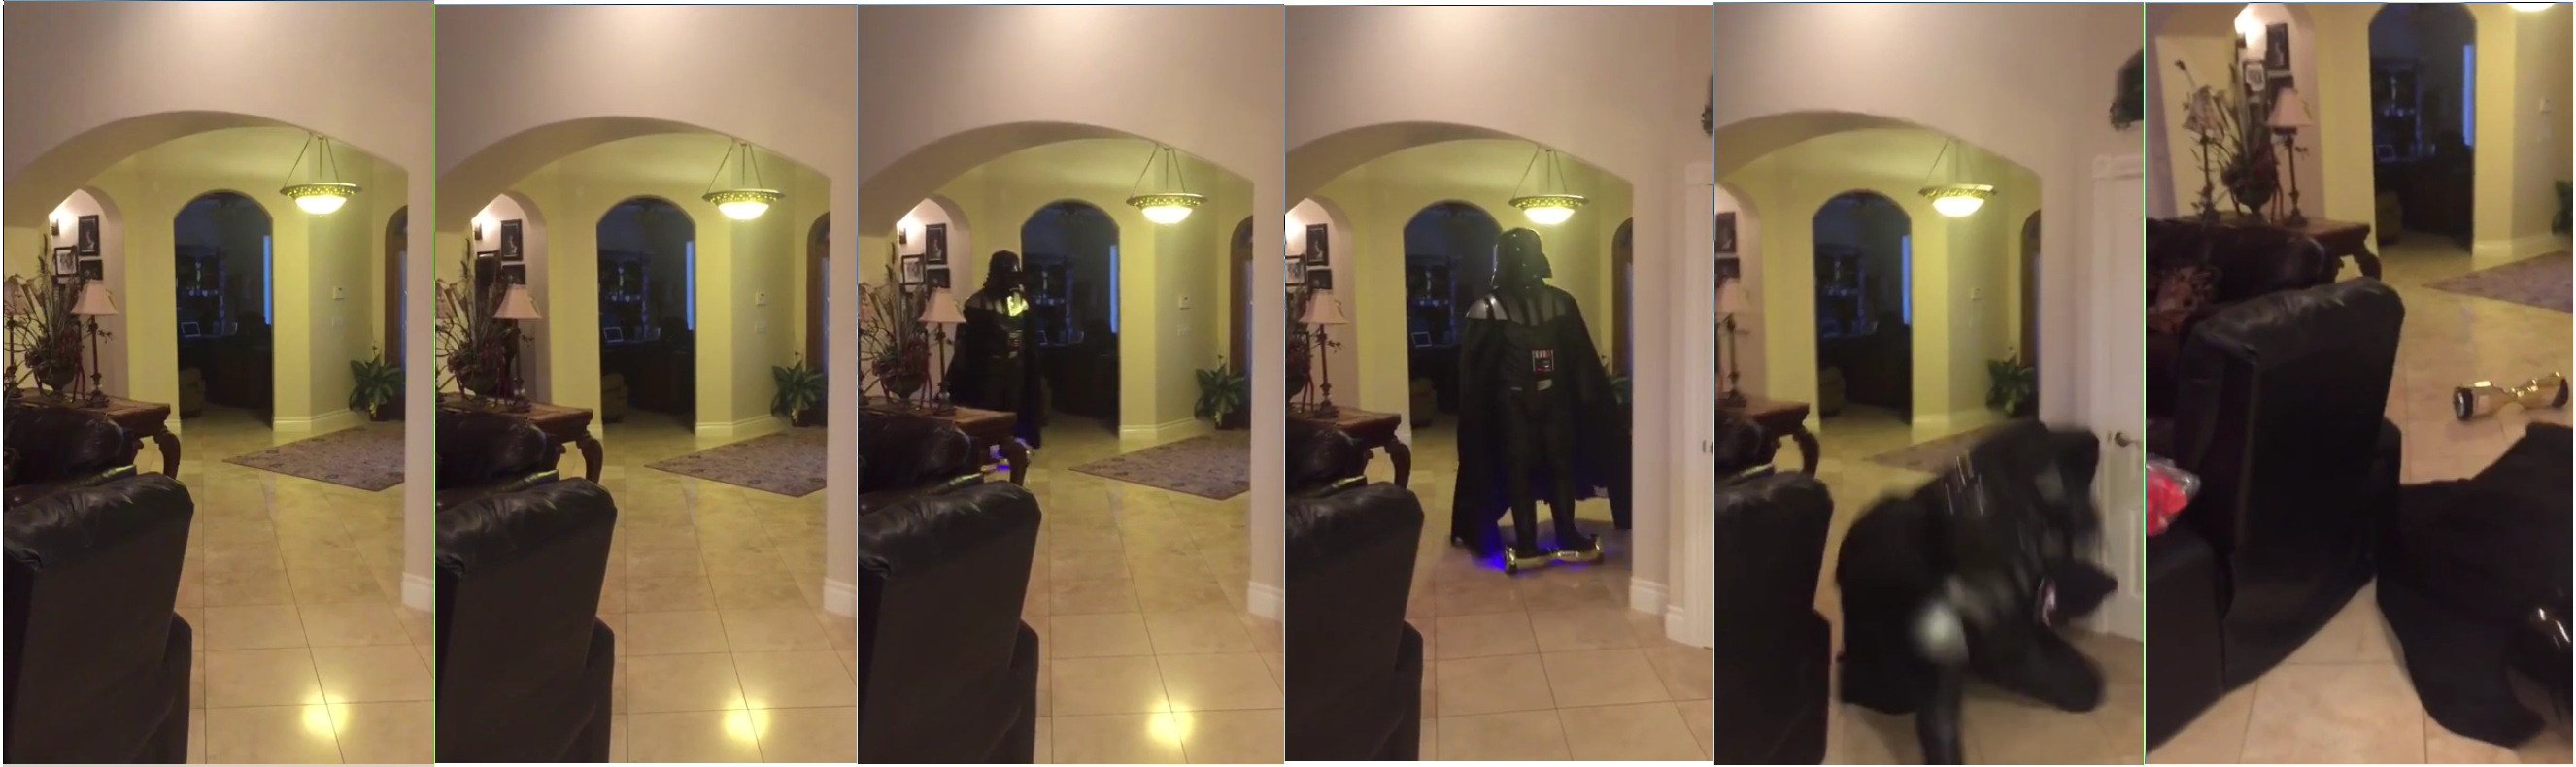
\includegraphics[width=0.95\textwidth]{imgs/resultados_error/recorrido.png}
    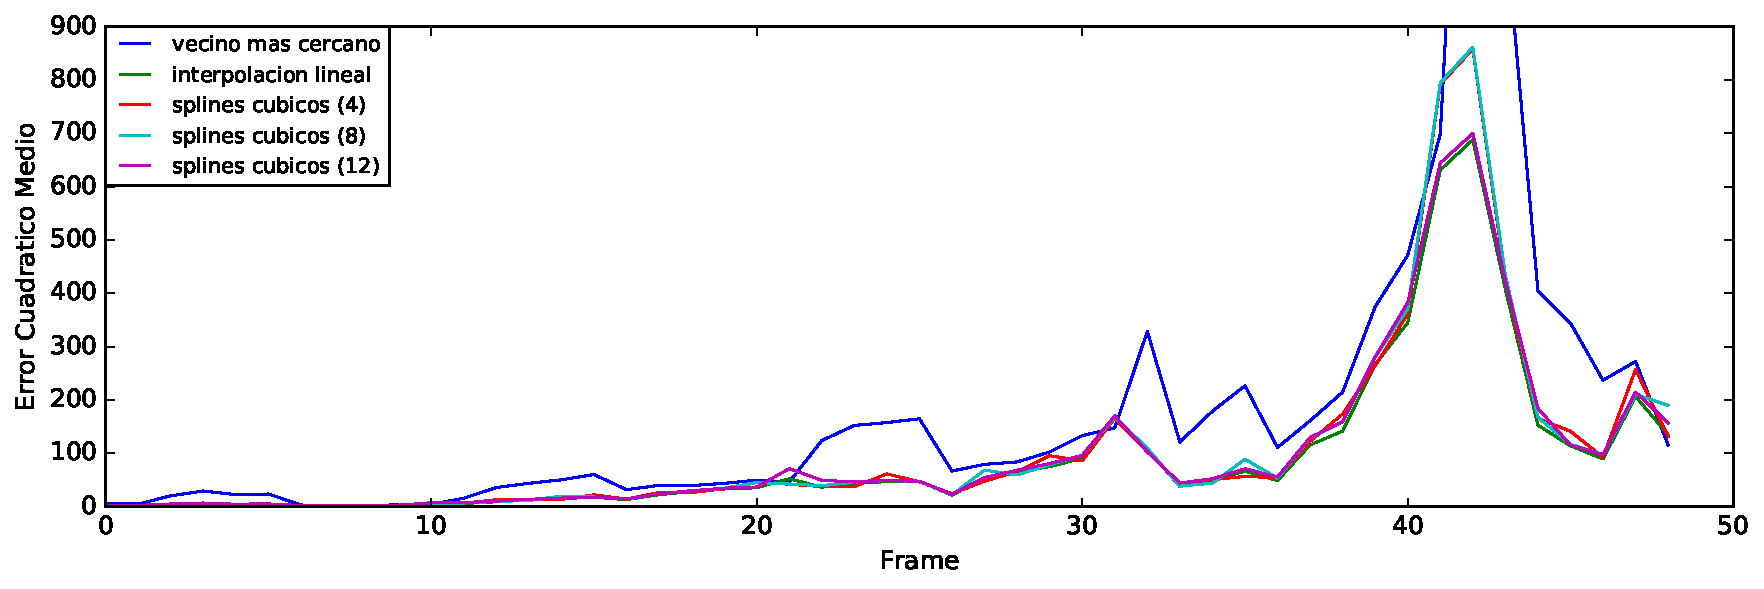
\includegraphics[width=1\textwidth]{imgs/resultados_error/temporal.pdf}
    \caption{Error Cuadrático Medio a lo largo del tiempo para los distintos algoritmos para el video \texttt{darthvader}. Además arriba se puede ver un extracto del video en ese momento.}
    \label{fig:errtiempo}
\end{figure}

Como podemos observar en la figura \ref{fig:errtiempo}, al principio del video, los frames son prácticamente iguales, entonces el error en todos los algoritmos es muy bajo, dado que interpolar es básicamente repetir el frame.

Cuando aparece en escena el objeto que se mueve, el error aumenta. Sin embargo, como la velocidad a la que se mueve es muy baja, el error sigue siendo relativamente medio-bajo. 

Luego, cuando Darth Vader tropieza y se cae, el error asciende mucho. Esto se debe a que el movimiento es mucho, entonces interpolar se vuelve más dificil, y aparecen artifacts, dado que nuestros algoritmos no hacen seguimiento de objetos, sino que simplemente interpolan píxel a píxel.

Finalmente, la cámara se mueve un poco, generando error más bajo que antes, aunque sigue siendo alto, por la misma razón de la que se habló anteriormente.



